\chapter{A Code Transformation Paradigm for MDO Frameworks}
\label{sec:code_transformations}

\section{Overview and Definitions}

In recent years, several advanced scientific computing techniques have proliferated that offer fundamentally new capabilities by using non-standard interpretations of numerical code. Examples of these techniques include:

\begin{itemize}[noitemsep]
    \item Automatic differentiation \cite{griewank_automatic_1988}, a technique that allows efficient and accurate evaluation of a function's gradient at runtime
    \item Automatic sparsity detection \cite{gebremedhin_efficient_2009}, a technique that identifies which of a function's outputs may be affected by each input
    \item Automatic problem transformations (in the context of numerical optimization), including techniques such as:
    \begin{itemize}[noitemsep]
        \item Problem scaling \cite{nocedal_numerical_2006}, to improve the conditioning of Hessians and linear sub-problems
        \item Log-transformations of variables, constraints, and objectives (similar to geometric programming) \cite{kirschen, agrawal_disciplined_2019}, which can improve convexity or eliminate nonlinearities
        \item Redundant constraint elimination
    \end{itemize}
    \item Common subexpression elimination \cite{casadi}, where repeated calculations are automatically identified and rewritten for faster speed via pre-computation
    \item Backend-agnostic programming, which can enable hardware accelerators (e.g., GPUs), different math library backends, just-in-time (JIT) compilation, and automatic vectorization \& parallelization \cite{jax}
\end{itemize}

In this work, we collectively call this set of computational techniques \emph{code transformations}. Formally defined, a code transformation is any operator that a) intercepts some representation of the user's original code at runtime, b) automatically applies some improvement based on analysis of the code itself, and c) returns this improved function to be executed in-place of the original.
%Code transformations are essentially the union of two related existing computer science concepts: compiler optimizations and scientific machine learning.

This definition is similar to that of a ``compiler optimization'', though a distinction can be drawn in the implied level of code abstraction where the improvement is applied. Compiler optimizations typically refer to lower-level improvements at the level of source code static analysis or a language-level syntax tree (e.g., dead-code elimination, loop fusion, and static type inference and specialization). By contrast, code transformations broaden this to also include improvements at the higher level of computational graphs dynamically constructed within domain-specific modeling languages, or at the level of a data structure describing a complete numerical method (e.g., an optimization problem formulation).

Several of these higher-level transformations have recently been described using the related term of ``scientific machine learning'' (SciML) \cite{ma_modelingtoolkit_2021, hu_taichi_2018, lavin_simulation_2022}. This is particularly true for end-to-end automatic differentiation of physical simulators, which are then used for machine learning applications such as parameter estimation, surrogate modeling, or scientific hypothesis testing via probabilistic programming. Therefore, SciML methods can be seen as a subset of code transformation techniques that emphasize differentiability and compatibility with machine learning frameworks; often, SciML implementations make various engineering tradeoffs that favor this goal \cite{rackauckas_engineering_2021}.

%as well as the composability of such transformations through their expression as higher-order functions \cite{jax}. A beneficial consequence of this dynamic, composability-first point of view has been the growth of modeling languages \cite{_modelica_2023, ma_modelingtoolkit_2021, _simulink_2020, fourer_ampl_1989} and domain-specific languages for machine learning \cite{pytorch, hu_taichi_2018}, which can offer reduced barrier to entry.

% separates declarative and imperative code; HTML/CSS,
% undersells impact—not just ml

In this way, code transformations can be roughly described as a union of both compiler optimizations and scientific machine learning. The benefit of introducing this broad ``code transformations'' abstraction is to recognize that all of these advanced techniques essentially share one major requirement to use: they require the ability to directly inspect some representation\footnote{In the general case of a code transformation, this must be a \emph{global} representation of the numerical problem} of the user's numerical code.

In practice, this code inspection can be done either via direct source code analysis or by constructing a computational graph of the numerical problem at runtime. The latter approach, which is called \textit{tracing} in machine learning literature \cite{jax, frostig_compiling_2018, baydin_automatic_2018}, is typically achieved by executing numerical code with a ``tracer'': a symbolic-like dummy data type that records operations performed on it. Where possible, this tracing approach is widely preferred to source code transformation\footnote{Maclaurin provides a comprehensive discussion of the tradeoffs between these techniques, and why tracing is often preferable in practice \cite{maclaurin_modeling_2016}}. Fortunately, modern syntactically-rich languages provide a variety of means to implement tracing, such as dynamic typing or multiple dispatch.

Where this tracing approach breaks down is when data structures are forcibly type-cast -- this causes the tracer to lose its recorded computational graph, and is referred to as ``breaking the trace''. The most common example where this might occur is across interfaces between programming languages -- for example, a


Therefore, for the purposes of this work, \textit{traceability} is effectively synonymous with code transformability.


A key observation is that many of these diverse techniques share similar principles. First, all of these techniques are operations that both act on and return executable code functions, and hence can be mathematically characterized as \emph{higher-order functions}.

This is because all of these techniques are operations that both act on and return executable code functions, and hence can be mathematically characterized as \emph{higher-order functions}.

Secondly,


%all of these advanced techniques essentially share one major requirement to use: the optimization framework must be able to inspect the actual code driving the design problem.


%Formally, we define a code transformation as:

%, where numerical code is written in a declarative style that separates numerics from execution. This includes
% Tradition ``compiler optimizations'' -> we look at them as a framework paradigm



%Here, we introduce the idea of \textit{code transformations} as a new computational paradigm on top of which an MDO framework can be built. Here, code transformations are defined as a generalized set of computational techniques that intercept the original optimization problem posed by the user (at runtime), apply some improvement based on analysis of the code itself, and then solve a modified optimization problem instead. This encompasses a variety of recent advanced techniques in scientific computing, such as:


The benefit of introducing this abstraction is to recognize that all of these advanced techniques essentially share one major requirement to use: the optimization framework must be able to inspect the actual code driving the design problem. This code inspection is done either via direct source code analysis or by creating a computational graph of the optimization model at runtime. The latter approach, which is called \textit{tracing} in machine learning literature \cite{jax, frostig_compiling_2018, baydin_automatic_2018}, is widely preferred to the former in modern, syntactically-rich languages\footnote{Maclaurin provides a comprehensive discussion of the tradeoffs between these techniques, and why tracing is often preferable in practice \cite{maclaurin_modeling_2016}}. Therefore, for the purposes of this work, \textit{traceability} is effectively synonymous with code transformability.

If code transformation techniques can be applied to engineering design optimization, they offer order-of-magnitude speedups over the black-box optimization methods that form the vast majority of industry use today \cite{martins_engineering_2021, lavin_simulation_2022}. These achievable speeds are comparable to those of state-of-the-art optimization methods in academia, such as disciplined optimization methods\footnote{such as geometric programming and disciplined convex programming} \cite{grant_disciplined_2006, gpkit, boyd_convex_2004, agrawal_disciplined_2019} and gradient-based methods using user-provided analytic gradients\footnote{sometimes referred to as ``adjoint methods'' in reference to a common method for manually deriving these gradients for more-complex analyses} \cite{gray_openmdao_2019, kenway_effective_2019, innes_don_2019}.

However, code transformations offer a key advantage over these state-of-the-art methods in that they can be applied \textit{automatically} -- most of the benefits of these advanced techniques can be gained without requiring any additional effort (or mathematical expertise) from the user. This ease-of-use is critical for practicality -- Grant notes that existing paradigms are hamstrung by a ``expertise barrier'' of existing methods, as described by Grant \cite{grant_disciplined_2006}. Table \ref{tab:paradigm_comparison} compares code transformations to existing MDO paradigms across three key practical metrics. In short, code transformations offer the best of both worlds: the computational speed of latest academic methods with the ease-of-use of methods already accepted by industry today.

\begin{table}[H]

    \newcolumntype{M}{>{\raggedright\arraybackslash}m{0.23\textwidth}}
    \newcolumntype{E}{>{\raggedright\arraybackslash}m{0.19\textwidth}}
    \newcolumntype{I}{>{\centering\arraybackslash}m{0.21\textwidth}}
    \newcolumntype{S}{>{\centering\arraybackslash}m{0.21\textwidth}}
    \newcolumntype{Q}{>{\centering\arraybackslash}m{0.16\textwidth}}

    \definecolor{q1}{HTML}{EC0505}
    \definecolor{q2}{HTML}{458505}
    \definecolor{q3}{HTML}{068383}
    \definecolor{q4}{HTML}{0C6CFD}

    \newcommand{\bad}{\textcolor{q1}{\large\textbf{Limited}}}
    \newcommand{\good}{\textcolor{q2}{\large\textbf{Good}}}
    \newcommand{\great}{\textcolor{q3}{\large\textbf{Great}}}
    \newcommand{\best}{\textcolor{q4}{\large\textbf{Best}}}

    \centering
    \caption{A subjective comparison of tradeoffs between existing MDO framework paradigms and the proposed \textit{code transformation} paradigm. The industrial state-of-the-art is largely \textit{black-box optimization}. The academic state-of-the-art has two major branches: \textit{gradient-based methods with analytical gradients}, and \textit{disciplined optimization methods}. More detailed discussion of these assessments, including definitions and reasoning, is given in Appendix \ref{chap:paradigm_comparison}.}
    \label{tab:paradigm_comparison}

    \begin{adjustbox}{width=\textwidth}
        \begin{tabular}{M E I S Q}
            \toprule
            \textbf{MDO Framework Paradigm}                 & \textbf{Example Frameworks and Tools}                                                                                                                                                                                                       & \textbf{Ease of \mbox{Implementation}}\ (idea-to-code) & \textbf{Runtime Speed and Scalability}\ (code-to-result) & \textbf{Modeling Flexibility} \\ \toprule
            \textbf{Black-box Optimization}                 & SUAVE \cite{SUAVE2017}, OpenMDAO$^*$ \cite{gray_openmdao_2019}, TASOPT \cite{drela_tasopt_2010}, PASS \cite{antoine_framework_2005}, FAST \cite{fast_ga_code}, FLOPS \cite{flops}, FBHALE \cite{fbhale}, \textbf{almost all industry codes} & \great & \bad & \best \\ \midrule
            \textbf{Gradient-based with Analytic Gradients} & MACH-Aero \cite{he_aerodynamic_2018}, OpenMDAO$^*$ \cite{gray_openmdao_2019}, OpenConcept \cite{brelje_multidisciplinary_2021} & \bad & \best & \great \\ \midrule
            \textbf{Disciplined Optimization}               & GPkit \cite{gpkit}, other convex methods \cite{karcher_method_2023, boyd_convex_2004, grant_disciplined_2006}, most algebraic modeling languages & \good & \good & \bad \\ \midrule
            \textbf{Code \mbox{Transformations}}            & AeroSandbox$^\dag$ \cite{sharpe_aerosandbox_2021}, JAX$^\ddag$ \cite{jax}, ModelingToolkit.jl$^\ddag$ \cite{ma_modelingtoolkit_2021} & \good & \great & \good \\
            \bottomrule

            \multicolumn{5}{p{1\textwidth}}{$^*$ Can use either paradigm, depending on user's implementation} \\
            \multicolumn{5}{p{1\textwidth}}{$^\dag$ Part of the present work, as detailed in Section \ref{sec:code_transformations}} \\
            \multicolumn{5}{p{1\textwidth}}{$^\ddag$ These are computational tools to facilitate code transformations, rather than frameworks themselves}
        \end{tabular}
    \end{adjustbox}

\end{table}

This leads to a compelling value proposition: if we can develop new methods for industry engineers to easily write traceable design code, then we gain access to an host of advanced scientific computing techniques that can significantly shrink the academia-industry MDO gap described in Chapter \ref{chap:literature}.

Thus, this contribution is twofold. First, the thesis will conceptually introduce code transformations as a new paradigm for engineering MDO frameworks. Secondly, the thesis will demonstrate strategies that allow traceability of engineering design code with minimal user effort, enabling the use of code transformations in practice.

\section{Results-To-Date in Code Transformations}


To explore and demonstrate this code transformation paradigm, we created \textit{AeroSandbox}, a Python-based MDO framework for conceptual design. This framework serves as both a proof-of-concept implementation as well as a proving ground for testing new transformations, with specific focus on engineering design applications. On top of this code framework, many optional aircraft-design-specific tools and physics modules are included; nevertheless, the core design optimization framework is applicable for conceptual design of many large-scale engineering systems. The code is made available open-source on GitHub under the permissive MIT license in order to gather as much practical user feedback as possible.

Core components of this framework and its mathematical basis are discussed more fully by Sharpe \cite{sharpe_aerosandbox_2021}. The framework is built on top of the \textit{CasADi} \cite{casadi} and \textit{JAX} \cite{jax} scientific computing libraries, which allow the computational graph tracing and several of the code transformation capabilities that are central to this work. The framework is designed to be modular and extensible, with a focus on ease-of-use and interpretability. The framework is also designed to be highly performant, with a focus on leveraging code transformations to achieve high computational speeds. As an optimization backend, the framework currently solves the transformed optimization problem using IPOPT, a primal-dual interior point algorithm \cite{wachter_implementation_2006}.

Fundamentally, AeroSandbox is a tool for building and transforming computational graphs, and indeed these graphs can be directly inspected both computationally and visually, as Figure \ref{fig:computational-graph-aerosandbox} shows. When constructing this graph, AeroSandbox deliberately makes certain framework-level decisions (e.g., to use a static, rather than dynamic graph; to use heuristics for forward- vs. reverse-mode automatic differentiation); these choices are tradeoffs that tend to work well on engineering analysis code \cite{rackauckas_engineering_2021}.

\begin{figure}[h]
    \centering
    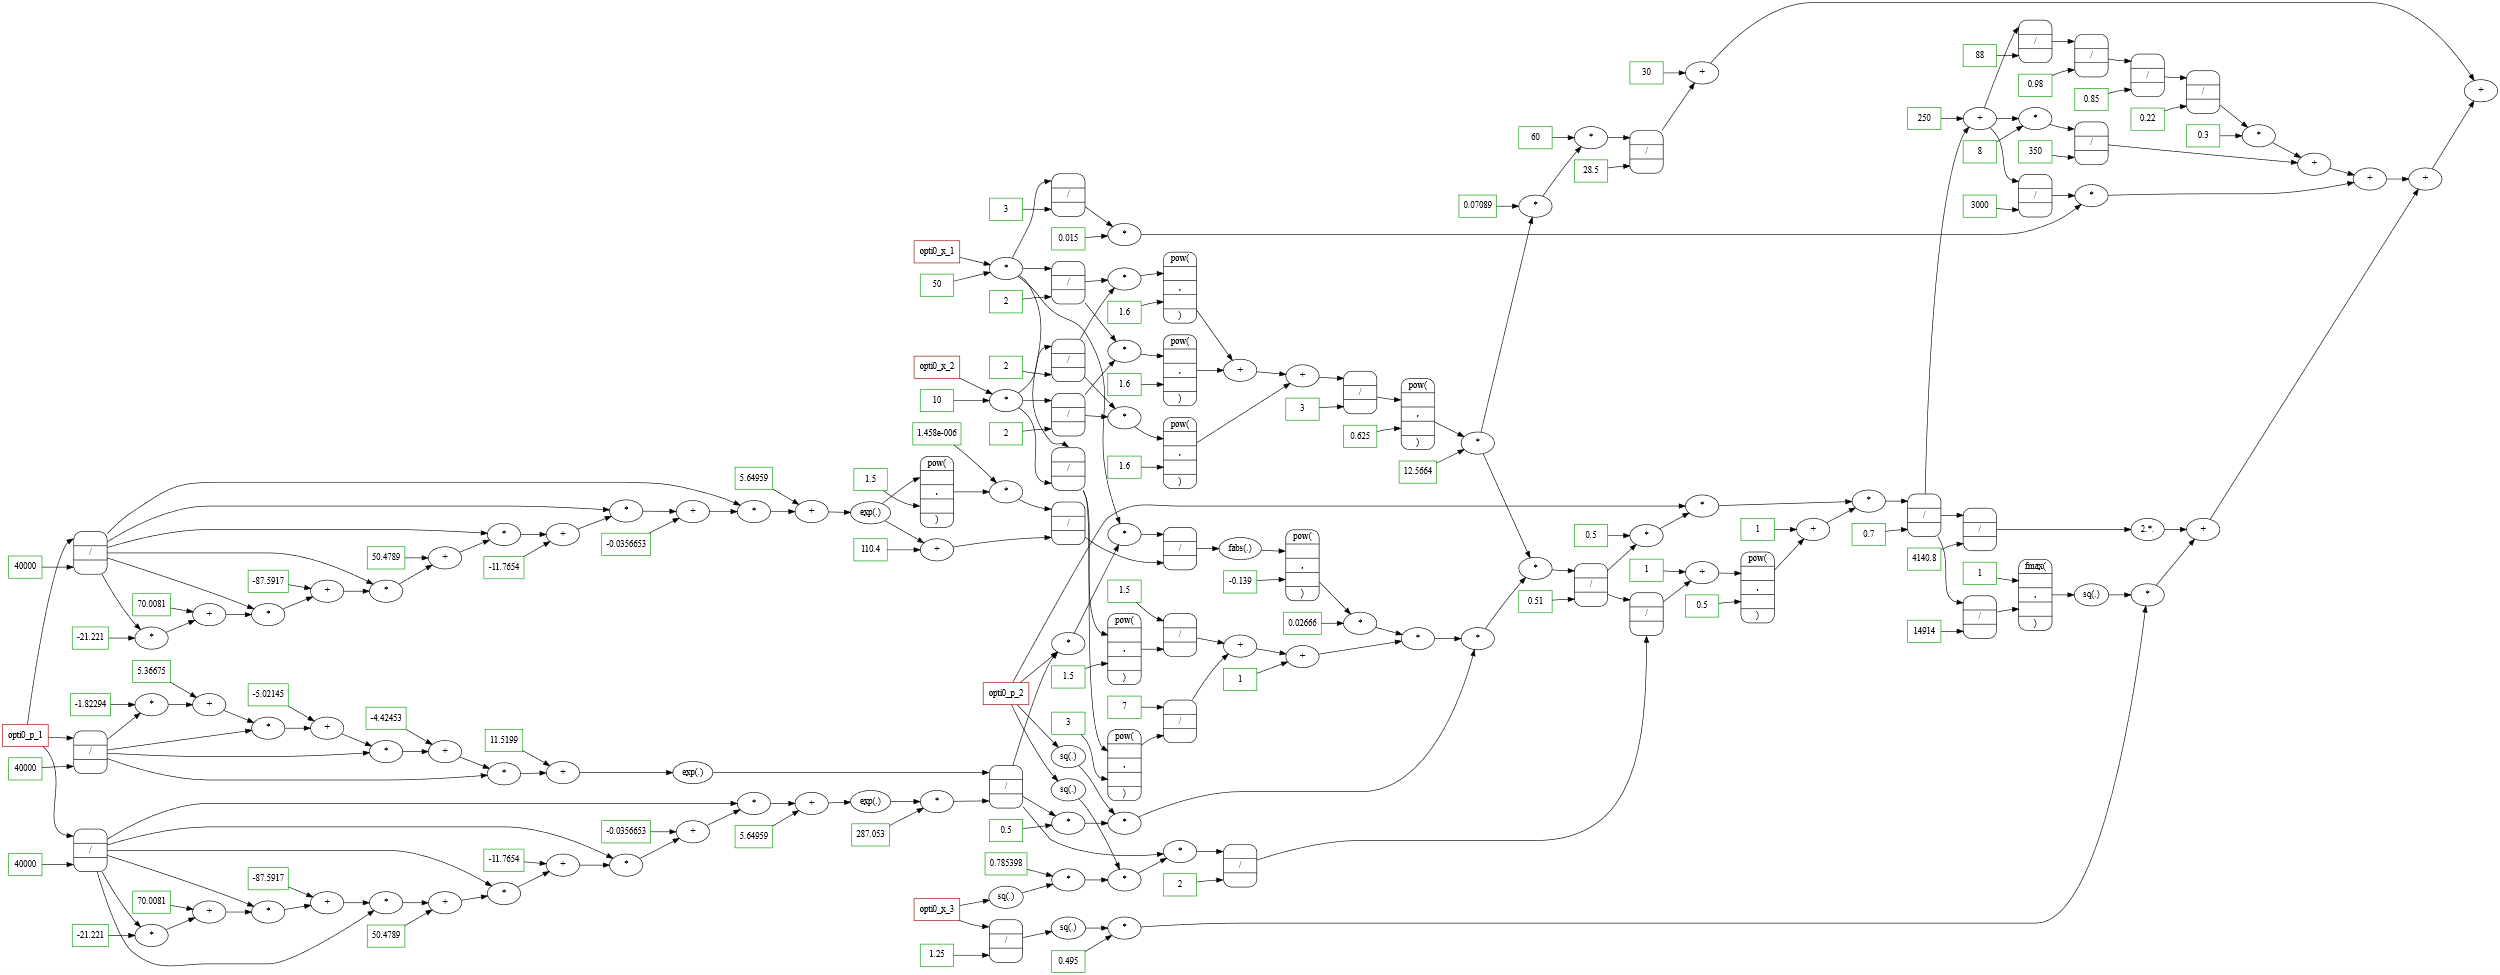
\includegraphics[width=\textwidth]{../figures/computational_graph_blimp.png}
    \caption{Computational graph of a mass model for an airship, as constructed by AeroSandbox. This graph is automatically constructed at runtime.}
    \label{fig:computational-graph-aerosandbox}
\end{figure}

AeroSandbox can be used to demonstrate the potential of code transformations to accelerate optimization problems with minimal effort. Here, we give an example comparison using the Rosenbrock optimization problem. This problem is a classic optimization benchmark, designed to be a stress-test as the optimum lies at the bottom of a shallow-curving valley \cite{rosenbrock}. Here, we solve an $N$-dimensional extension of this problem, which conveniently gives a knob to dial up or down the difficulty of the problem \cite{kok}. This optimization problem is defined in Equation \ref{eq:rosenbrock}:

\begin{mini}
    |l|
        {\vec{x}}{ \sum_{i=1}^{N-1} \left[ 100 \left(x_{i+1} - x_i^2 \right)^2 + \left(1 - x_i \right)^2 \right] }
        {}{}
%        \addConstraint{}
    \label{eq:rosenbrock}
\end{mini}

Figure \ref{fig:rosenbrock} illustrates this optimization landscape for the case where $N=2$, showing the curved valley. For all $N$, the global optimum is at $\vec{x} = \vec{1}$, where the objective function evaluates to $0$. This problem is chosen here because it shares many difficult aspects with engineering design optimization problems: it is nonlinear, nonconvex, and poorly-scaled. Furthermore, we deliberately choose poor initial guesses, with each element of the vector of initial guesses drawn from a random uniform distribution in the interval $[-10, 10]$.

\begin{figure}[H]
    \centering
    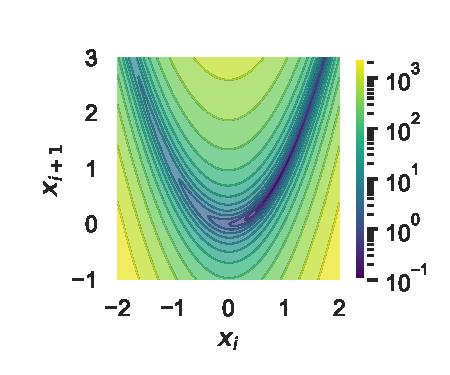
\includegraphics{../figures/rosenbrock_function.pdf}
    \caption{The Rosenbrock function, a classic optimization benchmark problem.}
    \label{fig:rosenbrock}
\end{figure}

In Figure \ref{fig:aerosandbox_scaling_comparison}, the performance of AeroSandbox (which leverages code transformations) is compared against existing methods using black-box optimization techniques. AeroSandbox offers faster practical and asymptotic optimization performance than existing black-box optimization methods, demonstrating the magnitude of acceleration that is possible with code transformations.

\begin{figure}[H]
    \centering
    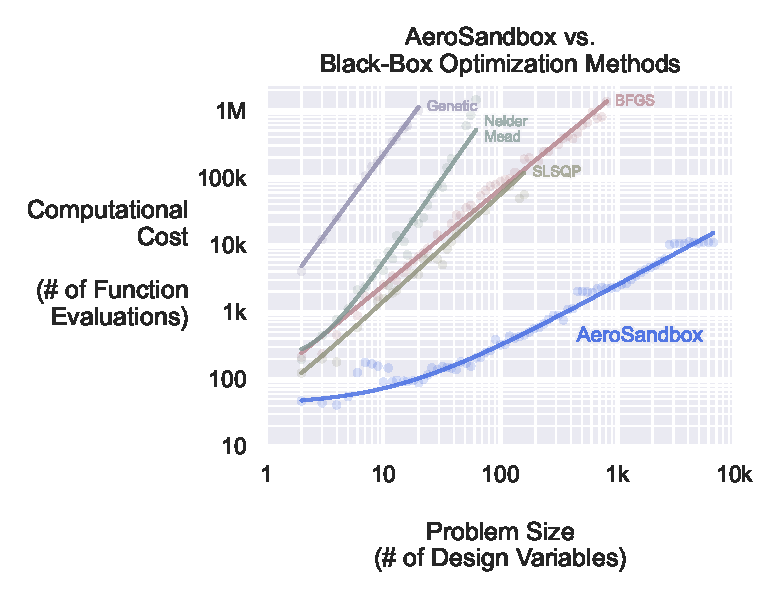
\includegraphics[width=0.8\textwidth]{../figures/benchmark_nd_rosenbrock.pdf}
    \caption{Comparison of optimization performance between AeroSandbox and existing black-box optimization methods on the $N$-dimensional Rosenbrock problem. Other methods are a Nelder-Mead simplex method and two gradient-based methods (SLSQP and BFGS), both using common SciPy implementations \cite{scipy}.}
    \label{fig:aerosandbox_scaling_comparison}
\end{figure}

Engineering benchmarks comparing the performance of an early implementation of the code transformations paradigm to disciplined optimization methods are given in Sharpe \cite{sharpe_aerosandbox_2021}. In short, code transformations can equal or exceed the performance of disciplined optimization methods such as geometric programming, even on problems where this disciplined optimization approach is applicable. This is a promising result, as it suggests that code transformations may be able to offer the best of both worlds on engineering problems: the computational performance of disciplined optimization methods without the strict mathematical restrictions.
